		We rewrite the conic \eqref{eq:chapters/12/6/5/27/curve} in matrix form.
    \begin{align}
        \vec{x}^\top\myvec{1&0\\0&0}\vec{x} + 2\myvec{0&-1}\vec{x} = 0
        \label{eq:chapters/12/6/5/27/curve-mtx}
    \end{align}
    Comparing with the general equation of the conic,
    \begin{align}
        \vec{V}_0 = \myvec{1&0\\0&0},\
        \vec{u}_0 = \myvec{0\\-1},\ 
        f_0 = 0 
    \end{align}
    Therefore, the equation of the normal where $\vec{q}$ is the point of contact 
    and 
\begin{align}
    \vec{R} \triangleq \myvec{0&-1\\1&0} 
\end{align}
is
    \begin{align}
	    \brak{\vec{V}_0\vec{q}+\vec{u}_0}^\top\vec{R}\brak{\myvec{0\\5}-\vec{q}} &= 0
        \label{eq:chapters/12/6/5/27/normal}
    \end{align}
    Substituting appropriate values and simplifying, we get 
    \begin{align}
	    \vec{q}^\top\myvec{0&1\\0&0}\vec{q} + 2\myvec{-2 & 0}\vec{q}= 0
        \label{eq:chapters/12/6/5/27/q-eqn}
    \end{align}
    which can be expressed as 
    \begin{multline}
	    \frac{1}{2}\lcbrak{
		    \vec{q}^\top\myvec{0&1\\0&0}\vec{q} + 2\myvec{-2 & 0}\vec{q}}
	\\
	    +
	    \rcbrak{
		    \vec{q}^\top\myvec{0&1\\0&0}^\top\vec{q} + 2\myvec{-2 & 0}\vec{q}}= 0
    \end{multline}
    yielding
    \begin{align}
	    \vec{q}^\top\myvec{0&\frac{1}{2}\\\frac{1}{2}&0}\vec{q} + 2\myvec{-2 &0}\vec{q} = 0
        \label{eq:chapters/12/6/5/27/q-affine}
    \end{align}
        \eqref{eq:chapters/12/6/5/27/q-affine}
	also looks like a conic with parameters
    \begin{align}
        \vec{V} = \myvec{1&0\\0&0},\
        \vec{u} = \myvec{0\\-1},\ 
        f = 0 
    \end{align}
The eigenparameters of $\vec{V}$ are
    \begin{align}
        \label{eq:chapters/12/6/5/27/PD}
        \vec{P} = \myvec{1&1\\1&-1},\ \vec{D} = \myvec{1&0\\0&-1}
    \end{align}
    Applying the affine transformation
    \begin{align}
        \label{eq:chapters/12/6/5/27/affine}
        \vec{q} &= \vec{Py} + \vec{c} \\
        \vec{c} &= -\vec{V}^{-1}\vec{u} 
 =\myvec{0\\4} \\
        f_0 &= \vec{u}^\top\vec{V}^{-1}\vec{u} - f 
            =  0
    \end{align}
$\because \det{V} = -\frac{1}{4} \neq 0$, 
	  using \eqref{eq:pair-cond},
        \eqref{eq:chapters/12/6/5/27/q-affine}
 represents a pair of straight lines.
      From \eqref{eq:pair-conic},
        \eqref{eq:chapters/12/6/5/27/PD},
	\eqref{eq:incircle-disc-v}
	and 
	\eqref{eq:incircle-disc-v-lam},
    \begin{align}
%        y_1^2-y_2^2 &= 0 \\
%        \implies y_1 &= \pm y_2 \\
%        \implies \vec{y} &= \myvec{a\\\pm a},\ a \in \mathbb{R}
\vec{y} = \kappa\myvec{1\\\pm 1}.
        \label{eq:chapters/12/6/5/27/y-sol}
    \end{align}
    Hence, using 
        \eqref{eq:chapters/12/6/5/27/affine},
    \begin{align}
        \vec{q} 
                = \myvec{0\\4}+\kappa\myvec{1\\\pm 1},
%                &= \myvec{a\pm a\\a\mp a+4} \\
        \label{eq:chapters/12/6/5/27/x-case}
    \end{align}
which, upon substituting in 
        \eqref{eq:chapters/12/6/5/27/curve-mtx}
	and solving for $\kappa$ yields
\begin{align}
	\kappa = \pm \sqrt{2}, -2.
\end{align}
 Thus, the points of contact are
    \begin{align}
        \vec{q}  = \cbrak{\myvec{\pm 2\sqrt{2}\\4},\myvec{0\\0}}
        \label{eq:chapters/12/6/5/27/poc-ans}
    \end{align}
    The nearest point out of these three candidates for $\vec{q}$ is
    $\myvec{\pm2\sqrt{2}\\4}$. 
See \figref{fig:chapters/12/6/5/27/normal}.
\begin{figure}[!ht]
        \centering
        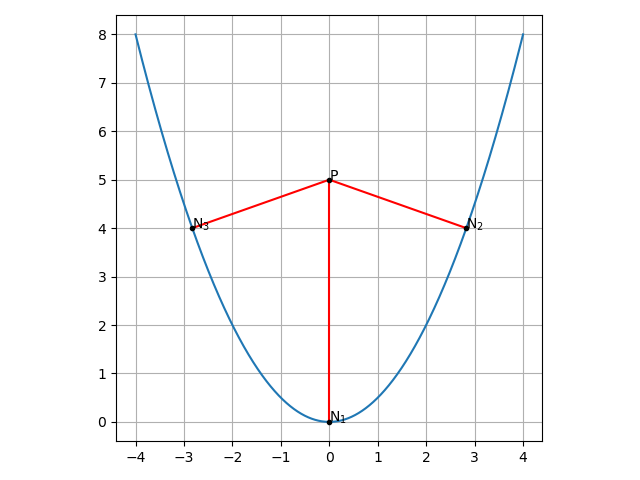
\includegraphics[width=\columnwidth]{chapters/12/6/5/27/figs/normal.png}
        \caption{}
        \label{fig:chapters/12/6/5/27/normal}
    \end{figure}
